\documentclass{standalone}

\usepackage{tikz}
\usepackage{circuitikz}

\tikzset{block/.style = {draw, fill=white, very thick, rectangle, minimum height=1cm, minimum width=2cm},
         lblock/.style={draw,fill=white,very thick, rectangle, minimum height=3cm, minimum width=1cm},
         sum/.style= {draw, fill=white, very thick, circle, node distance=0.5cm}}

         
\begin{document}
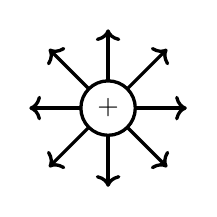
\begin{tikzpicture}[scale=2]
\draw[<->, very thick](-0.5,0)--(0.5,0);
\draw[<->, very thick](0,-0.5)--(0,0.5);
\draw[<->, very thick](-0.375,-0.375)--(0.375,0.375);
\draw[<->, very thick](0.375,-0.375)--(-0.375,0.375);
\node[sum](+)at(0,0){$+$};
\end{tikzpicture}
\end{document}